\documentclass[]{IEEEtran}
\IEEEoverridecommandlockouts
\usepackage{cite}
\usepackage{amsmath,amssymb,amsfonts}
\usepackage{graphicx}
\usepackage{textcomp}
\usepackage{xcolor}
\usepackage{multirow}
\usepackage{url}
\usepackage{booktabs}
\usepackage{float}
\usepackage{hyperref}
\usepackage{balance}

\hypersetup{
  pdftitle={A Ball-on-Arc Benchmark: Classical and Learning-Based Control on Realistic Deployment Hardware},
  pdfauthor={Jaydeepkumar Ranpariya; Sandipan Nath; Alexander Mattick; Georgios Kontes; Tobias Feigl; Christopher Mutschler},
  pdfsubject={arXiv preprint}
}

\newcommand{\setupimg}{figures/system_setup.jpg}

\begin{document}

\title{A Ball-on-Arc Benchmark: Classical and Learning-Based Control\\on Realistic Deployment Hardware}

\author{
\IEEEauthorblockN{
  Jaydeepkumar Ranpariya, Sandipan Nath, Alexander Mattick,\\
  Georgios Kontes, Tobias Feigl, and Christopher Mutschler}
\IEEEauthorblockA{
  Fraunhofer Institute for Integrated Circuits IIS, Nuremberg, Germany}
\IEEEauthorblockA{
  \{jaydeepranpariya037@gmail.com, sandipan.nath@fau.de,\\
  alexander.mattick@iis.fraunhofer.de\}}
}

%% ORCIDs: Ranpariya 0009-0000-1967-9795; Nath 0009-0008-4830-6451;
%% Mattick 0000-0001-7805-199X; Kontes 0000-0001-7051-0960;
%% Feigl 0000-0002-3040-3543; Mutschler 0000-0001-8108-0230.

\maketitle

\begin{abstract}
Reproducibility and fair comparison of control paradigms, i.e., classical,
predictive, and learning-based, in robotics research are widely called for,
yet controllers from different paradigms are seldom evaluated on the same
physical system under the same conditions. The aim of this article is to
provide a reproducible benchmark for comparing control paradigms on realistic
robot hardware. We built a compact ball-on-arc balancer that pairs an
industrial servo and motion controller with commodity sensors. We deliberately
keep real-world imperfections that a deployed controller must deal with to
enable a solid and realistic evaluation of controllers. We tested 13
controllers across four families under one common protocol. The hardware and
setup, the implemented controllers, and all trial records are publicly
available to foster reproduction of the results and to serve as a benchmark in
robotics research.
\end{abstract}

\begin{IEEEkeywords}
Robotics benchmarking, reinforcement learning, model predictive control,
ball balancing, sim-to-real transfer, learned dynamics models,
reproducible research
\end{IEEEkeywords}

\section{Introduction}
\label{sec:intro}

Robots are leaving the laboratory for factories and commercial sites, where a controller has to work in a realistic environment.
Deployed machines are assembled from parts chosen for cost and availability, so a precise industrial actuator often sits behind cheap sensors, or the other way around.
Picking a controller for such a machine is as much a practical question as a theoretical one.
Each option asks for something different up front: a classical law needs a model derived and tuned, a policy trained in simulation needs a simulator worth trusting, and a method learned from logs needs the logs collected on the machine.
Some of them also require online compute.
Model-based and learning-based control have both come a long way, so this is a real choice, and getting it wrong costs months of engineering.

The rigs built for benchmarking often smooth away the frictions of a realistic deployment~\cite{quanser_qube2}, so doing well on such a platform says little about how a controller would behave once deployed.
Nor do the comparisons themselves settle the choice, because methods are seldom measured against each other under the same conditions.
Most benchmarking stays inside a single family: classical controllers compared with other classical controllers, learning methods with other learning methods~\cite{wellstead1978ballbeam,ho2010smc,mahmood2018benchmarking,guertler2023benchmarking}.
The comparisons that reach across paradigms run in simulation~\cite{yuan2022safecontrolgym,akki2025benchmarking}, where the actuator and the sensors behave the way the simulator says they do.
The one that reaches hardware shares a rig and a protocol but lets each team tune its own entry, so tuning and method are measured together~\cite{wiebe2025reinforcementlearningrobustathletic}.

\begin{figure}[t]
  \centering
  \includegraphics[width=0.9\columnwidth]{\setupimg}
  \caption{The ball-on-arc platform: a freely rolling ball on a shallow arc,
    carried by a motorized linear cart.}
  \label{fig:setup}
\end{figure}

Our main goal is to provide a reproducible hardware benchmark that allows for the replication of our results and the evaluation of other control strategies in a realistic deployment scenario.
We built it around a ball rolling freely on a shallow arc carried by a motorized cart (Fig.~\ref{fig:setup}), where a controller steers the ball only indirectly, by moving the cart, until the ball balances at the center.
The task is small and underactuated, and quick enough to run and reset that a full 13-controller benchmark fits into a few sessions at the rig.

We drive the cart with an industrial servo through a belt, commanded via velocity; we track the ball with commodity sensors slower and noisier than what an ideal setup gives you; and the workspace has hard rail limits.
These frictions are ordinary in a deployed machine and usually engineered out of a benchmark rig, and on this platform every controller has to face them~\cite{dulac2021challenges}.

We ran thirteen controller configurations on the platform through the same four-state, scalar-command interface, each prepared the way its own paradigm asks (Tbl.~\ref{tab:controllers}).
We group them as classical feedback (PD, LQR, and sliding-mode control), predictive control (MPC and NMPC), reinforcement learning trained in simulation (PPO~\cite{schulman2017proximal}, TD3, TQC, SAC, and TRPO), and methods built from logged hardware data, which either plan through a learned dynamics model with Model Predictive Path Integral control (MPPI~\cite{williams2017mppi}), train a policy inside one (PPO-WM), or learn a policy straight from the logs with Implicit Q-Learning (IQL~\cite{kostrikov2022iql}).
We put each through the same 50-trial protocol from the same distribution of starting conditions, giving 650 hardware trials, and scored them on success rate, settling time, and control effort.
Because we held the conditions identical throughout, the differences that emerge are not artifacts of the setup, though each pipeline still brings its own model, tuning, and boundary handling.

In our trials, handling the boundary mattered more than the choice of controller family for reliability.
Each of the three classical controllers corrects the ball, but doing so drives the cart to the end of the rail, where it cannot recover, and most of their trials fail.
Adding a wall override without changing the gains lifts all three into the reliable group.
Once the boundary is handled, every family has a controller that rarely fails.
The families differ more on speed and effort, and there the clearest advantage came from learning a dynamics model on hardware data.
Planning through such a model, MPPI succeeds on every trial, settles fastest, and uses the least control effort, in exchange for running model rollouts inside every control period.
The protocol resolves only large differences, so we avoid reading a ranking into small ones.

For reproducing the comparison and extending the platform, we release the hardware design, the controller implementations, the trained models, the random-exploration datasets, and the complete trial record.\footnote{\url{https://github.com/JDRanpariya/ball-balancing-on-arc}}

The remainder of this article is organized as follows.
Sec.~\ref{sec:related} positions the platform against prior work, Sec.~\ref{sec:system} describes the system, and Sec.~\ref{sec:controllers} the controllers.
Sec.~\ref{sec:experiments} defines the evaluation protocol, Sec.~\ref{sec:results} reports the results, and Sec.~\ref{sec:discussion} distills the takeaways for practitioners.

\section{Related Work}
\label{sec:related}

Comparisons of control methods have become rigorous within each family, yet they rarely reach across them.
The ball-and-beam and its ball-on-arc relatives have served as control testbeds since the 1970s, usually one controller at a time~\cite{wellstead1978ballbeam}.
Real-robot benchmarking has since become far more systematic, though mostly within reinforcement learning: a systematic evaluation of RL on physical robots compares model-free algorithms with one another~\cite{mahmood2018benchmarking}, with classical and predictive control outside its scope.
Control learned from data, whether by planning through a learned dynamics model, training a policy inside one, or fitting a policy offline from logged data, forms a substantial line of its own, and its hardware evaluations stay within it too, as in an offline-RL benchmark on manipulation hardware~\cite{guertler2023benchmarking}.
The efforts that do span paradigms, most notably safe-control-gym, which evaluates classical control, MPC, and RL under shared constraints~\cite{yuan2022safecontrolgym}, and a comparison of MPC and RL for legged locomotion~\cite{akki2025benchmarking}, run in simulation.

When multi-method comparison does reach hardware, it tends either to idealize the plant or to split the tuning across authors.
The classic rigs, with the Quanser rotary servo pendulum as a representative example~\cite{quanser_qube2}, pair a direct-drive motor and clean encoders with a closely matched simulator, so little of the sim-to-real gap a deployed system faces ever reaches the bench.
The closest effort on hardware, the second AI Olympics on the RealAIGym underactuated double pendulum~\cite{wiebe2025reinforcementlearningrobustathletic}, runs on real quasi-direct-drive hardware under a shared protocol.
Its four finalists are all reinforcement-learning variants, each authored and tuned by a separate team, so its comparison stays within reinforcement learning rather than spanning the classical, predictive, and learning-based paradigms, and its quasi-direct-drive plant leaves out the actuation and sensing frictions of a deployed rig.
An empirical study of real-world reinforcement learning identifies latency, noise, and constraints among the conditions where learning-based controllers most often fail~\cite{dulac2021challenges}.

Those are the conditions a benchmark should put a controller through, yet no shared hardware bench presents them to every paradigm at once.
A comparison worth trusting also has to be reproducible: implementation and evaluation choices already dominate learning-based outcomes~\cite{henderson2018deeprl,agarwal2021precipice}, and on hardware the plant becomes one of those choices, since no two rigs share the same friction, latency, and sensor behavior, so the rig has to be documented well enough for another laboratory to rebuild it.
Bonsignorio and Zereik reached that bar for a two-method visual-servoing comparison on a low-cost arm~\cite{bonsignorio2021visualservoing}; doing the same across every paradigm, on hardware that keeps the frictions of deployment, is the harder task that remains.

\section{The Ball-on-Arc Platform}
\label{sec:system}

\begin{figure}[t]
  \centering
  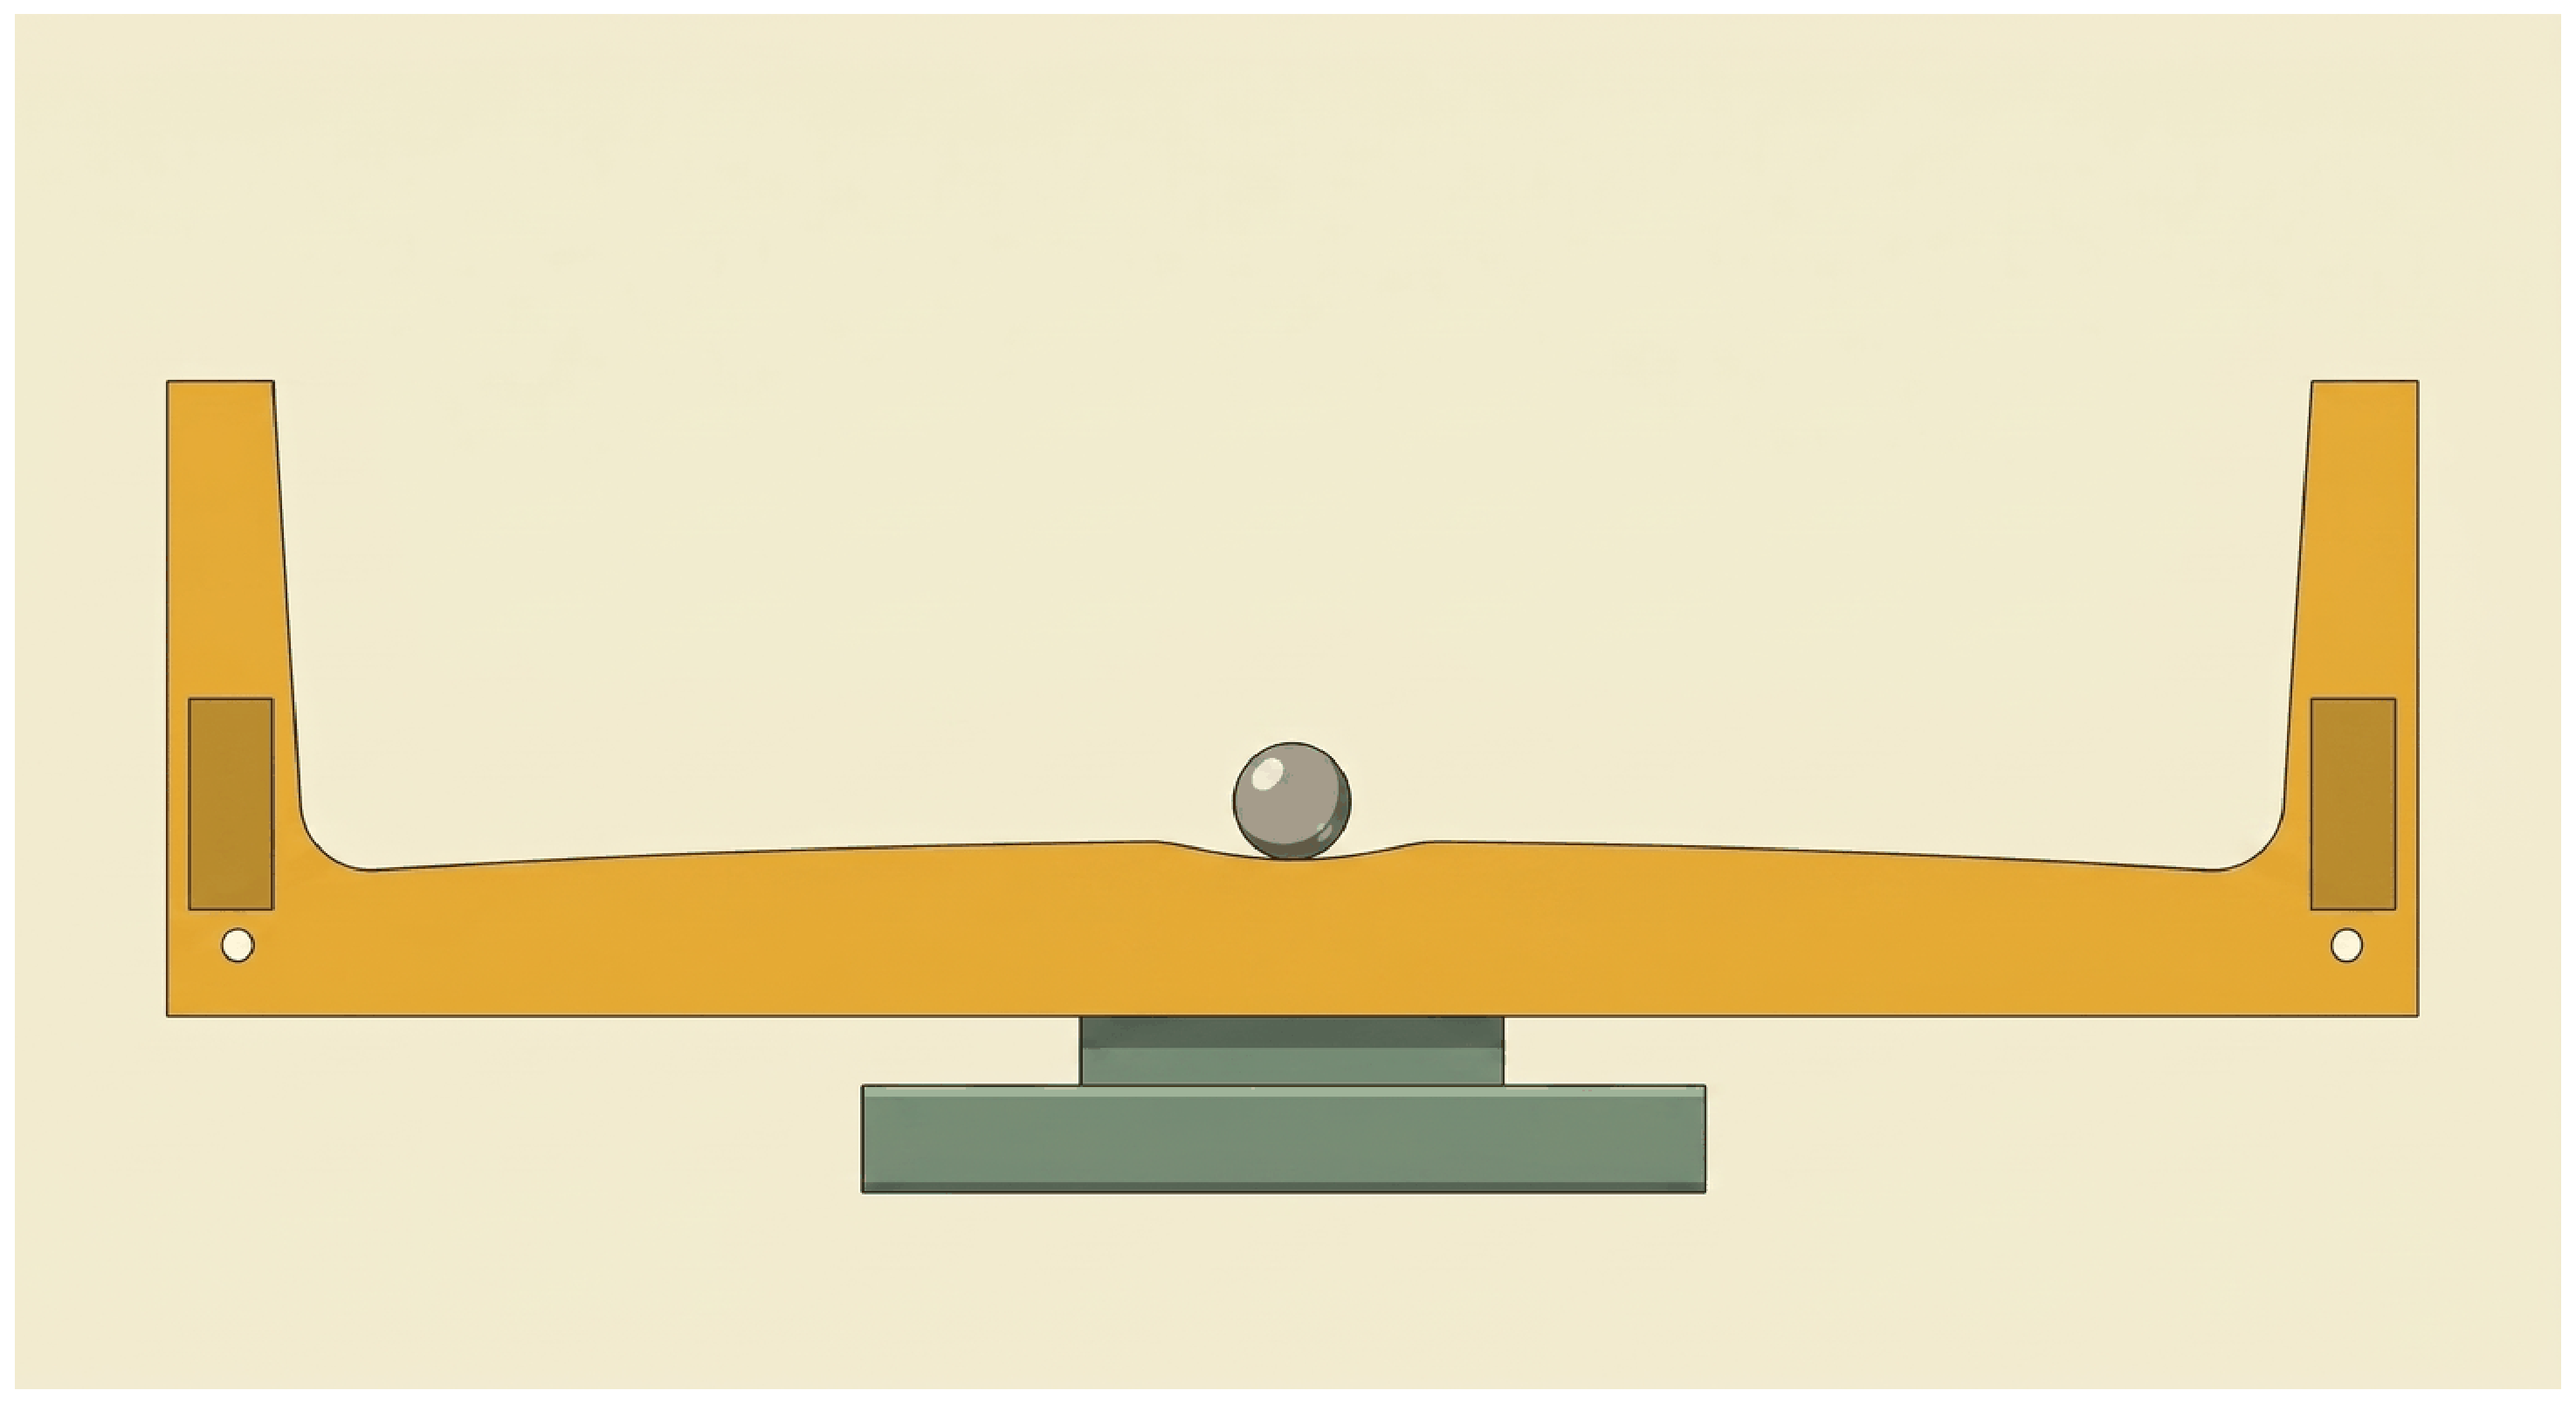
\includegraphics[width=0.9\columnwidth]{figures/ball_on_arc_cart.eps}
  \caption{Cross-section of the cart, a single 3D-printed part whose top
    surface is the arc the ball rolls on. A shallow concave dip at the
    center, where the ball rests, forms a weak but restoring
    gravitational well, so the balance point is locally stable and
    lightly damped. The cart rides the linear actuator below it and
    translates left and right to steer the ball.}
  \label{fig:sketch}
\end{figure}


Our platform is an underactuated ball-on-arc system with a rail-constrained industrial cart and realistic on-board sensing.
The ball is 24\,g and 9\,mm in radius, and the convex arc it rolls on has radius $R = 2.101$\,m with a shallow concave dip at its center (2\,mm deep, Fig.~\ref{fig:sketch}), mounted on a 3D-printed (PLA) cart\footnote{Printable STL models of the cart (with its integrated arc surface) and the mounts are included in the public repository.} riding a motorized linear actuator (Fig.~\ref{fig:setup}).
The dip forms a weak but restoring well, so the balance point is locally stable and lightly damped rather than open-loop unstable like the classical ball-and-beam, and a PD law holds the ball there with no integral term; the difficulty lies in the actuation, the sensing, and the rail.
The cart is moved by a rotary AC servo motor (Beckhoff AM8121) turning a belt-driven linear slide (SMC LEFB32NXS), commanded in velocity through an industrial EtherCAT servo drive (Beckhoff EL7201) under the TwinCAT motion runtime.
The actuator has 1.0\,m of physical stroke; its drive reports positions in axis units, in which the soft-limited workspace spans $\pm$0.78\,m.
All positions and velocities in this article use these axis units (the supplement gives the scaling).

Every controller reads the platform's own signals, with no observer reconstructing state: the ball angle straight from the time-of-flight geometry, its rate as a finite difference of that angle, and the cart's position and velocity from the servo encoder.
Whatever latency and noise the sensors carry therefore reaches each controller unfiltered.%; we quantify both below.

Recovering the ball is a textbook problem, but what makes this platform demanding are four frictions in the hardware:

\noindent\textbf{Underactuation:} The ball cannot be commanded directly, only indirectly by accelerating the cart, so an aggressive correction can destabilize the ball instead of recovering it.

\noindent\textbf{Hard constraints:} The workspace spans 1.56\,m in axis units, about 0.80\,m of the actuator's 1.0\,m stroke.
A controller that ignores the approaching boundary exhausts its maneuvering space on one side, limiting its ability to recover, which makes explicit constraint handling a central design concern on this platform~\cite{brunke2022safe}.

\noindent\textbf{Sensing:} Ball position comes from two VL53L0X Time-of-Flight sensors read alternately; in operation the estimate refreshes every ${\sim}$80--100\,ms (about 10--12\,Hz), well slower than the 50\,ms (20\,Hz) control loop, so the controller acts on ball measurements up to about two control cycles (${\sim}$100\,ms) old while the cart encoder updates synchronously.
Near the arc edge ($|\theta| > 0.071$\,rad), where the ball rolls within a few millimeters of a sensor, the reading enters the VL53L0X near-field \emph{blind zone} and saturates, holding at the boundary until the ball returns.
Even at center the ball-position reading varies about 13\,mm peak-to-peak ($\sigma \approx 3.3$\,mm; the raw per-unit spread is 14--17\,mm), so every controller has to cope with this noise and latency on its own.

\noindent\textbf{Velocity interface:} We command a velocity setpoint (\texttt{MC\_MoveVelocity}) within the axis limit of $\pm$0.9\,m/s, and the drive realizes it through an internal S-curve profiler and the servo's cascaded position, velocity, and current loops.
We model this as a first-order lag ($\tau_v = 0.15$\,s) for control design; the profiler, the inner loops, and the belt compliance do not appear in an open-loop simulator, and contribute to the platform's sim-to-real gap.

The state vector is 4-dimensional: cart position and velocity, ball angle and angular velocity; the control input is a scalar velocity command.
The complete dynamics equations and system parameters are provided in the supplementary material.

\section{The Controllers}
\label{sec:controllers}

We implemented 13 controllers (Tbl.~\ref{tab:controllers}), each meeting the platform through the same interface: it reads the current state and the physical limits, and returns a velocity command.
Holding that interface fixed keeps the comparison on the control law.
All numerical parameters, training configurations, and reward functions are detailed in the supplementary material.

\begin{table}[t]
\centering
\caption{The 13 benchmarked controllers. Paradigm labels follow
  standard taxonomy in control and RL literature. The taxonomy has two axes:
  data/model source (analytical model, simulation, hardware logs) and
  decision mechanism (feedback law, MPC/planning, online RL policy, offline RL policy).
  Suffixes: WO = wall override, DR = domain randomization, BZ = blind-zone sensor model,
  WM = learned world model.}
\label{tab:controllers}
\setlength{\tabcolsep}{3pt}
\footnotesize
\begin{tabular}{lll}
\toprule
\textbf{Controller} & \textbf{Data source} & \textbf{Decision mechanism} \\
\midrule
PD + WO        & Analytical model     & Error feedback + tuned gains \\
LQR + WO       & Analytical model     & PD-equivalent state feedback \\
SMC + WO       & Analytical model     & Sliding-mode feedback \\
\midrule
MPC + WO       & Analytical model     & Constrained QP planning \\
NMPC           & Analytical model     & Nonlinear MPC planning \\
\midrule
PPO (BZ+DR)    & Simulation           & Model-free RL (on-policy) \\
TRPO (DR)      & Simulation           & Model-free RL (on-policy) \\
SAC (DR)       & Simulation           & Model-free RL (off-policy) \\
TD3 (DR)       & Simulation           & Model-free RL (off-policy) \\
TQC (DR)       & Simulation           & Model-free RL (off-policy) \\
\midrule
PPO (WM)       & Logged data          & RL trained in learned model \\
MPPI           & Logged data          & Sampling MPC via learned model \\
IQL            & Logged data          & Offline model-free RL \\
\bottomrule
\end{tabular}
\end{table}

\subsection{Classical Control (PD, LQR, SMC)}

The three classical controllers follow the standard workflow: model, tune in simulation, deploy.
PD acts on measured position and velocity errors, LQR on the linearized dynamics, and SMC on a nonlinear sliding surface.
We tuned PD and SMC with CMA-ES~\cite{hansen2016cma}, an evolutionary optimizer, in simulation over stratified initial conditions.
For LQR, the CMA-ES-tuned gain does not transfer to the hardware, so we deploy a PD-equivalent gain instead; the supplement's classical-tuning appendix gives the details.
Each law is designed around the equilibrium and carries no notion of the rail ends from Sec.~\ref{sec:system}.

\noindent\textbf{The wall-override mechanism:} To give the nominal controllers a way to respect the boundary, we add a simple heuristic: when the cart approaches the rail limit, or wall, override whatever the nominal controller commands and drive away from it.
PD, LQR, SMC, and MPC all run with this guard, denoted ``+WO'' in our results; NMPC handles the rail through its own constraint formulation and runs without it.

\subsection{Predictive Control (MPC, NMPC)}

Linear MPC solves a constrained quadratic program (QP) at each timestep using linearized dynamics; NMPC uses the full nonlinear model over a horizon of $N=10$ steps.
Both were tuned with the same CMA-ES framework, in this case over cost weights and horizon parameters.
Near the rail, linear MPC's cart-position constraint can make that QP infeasible, so the deployed MPC~(+WO) drops the constraint and falls back on the same wall override as the classical controllers.

\subsection{Simulation-Trained Reinforcement Learning}

We trained five RL algorithms, PPO~\cite{schulman2017proximal}, TD3, TQC, SAC, and TRPO, in simulation with domain randomization.
The training environment includes the velocity interface of Sec.~\ref{sec:system}, so each policy trains against the servo dynamics the hardware presents; all use small two-layer MLPs, with architectures and training budgets in the supplement.
One variant, PPO (BZ+DR), also models the sensor blind zone of Sec.~\ref{sec:system} during training: with the simulated readings freezing near the arc edges as the real ones do, the policy learns to act cautiously while its inputs may already be stale.
We ablate this blind-zone model on PPO alone, comparing PPO with the sensor model against PPO without it (ablations in the supplementary material).

\subsection{Hardware-Data-Driven Controllers (IQL, MPPI, PPO-WM)}

These three controllers all learn from real hardware data, and each puts that data to work in a different way.

\noindent\textbf{Offline RL (IQL):} IQL~\cite{kostrikov2022iql} learns a policy directly from logged hardware data, requiring no simulator.
We trained it on approximately 333,000 transitions (1,415 trials) collected from every controller we ran on hardware (MPPI, NMPC, RL, MPC, PD, LQR, SMC, and earlier offline-RL checkpoints, though not the deployed IQL policy itself).
The dataset is mixed, 83\% successful episodes and 17\% failures, and rewards are recomputed offline from the logged states.
IQL extracts its policy conservatively, through expectile regression~\cite{kostrikov2022iql}, which keeps it clear of the distributional-shift instabilities common to other offline RL methods.

\noindent\textbf{Model-based planning (MPPI):} This approach learns the system's dynamics directly from hardware data: a two-layer LSTM trained to predict state transitions from a 1M-transition random-exploration dataset.
At runtime MPPI treats this learned model as an internal simulator.
Every control step (50\,ms) it samples hundreds of candidate action sequences, rolls each forward through the network, and executes the first action of the cost-weighted-average sequence, replanning continuously as new data arrives.

\noindent\textbf{RL in a learned world (PPO-WM):} A second variant trains a standard PPO policy inside a learned world model~\cite{hafner2020dream} rather than using it for online planning.
The result is a lightweight network that trains and runs on CPU, with no GPU at deployment, while still drawing on dynamics learned from real data.
MPPI and PPO-WM share the same world-model architecture but were trained on two separate 1M-transition collections; the collection behind the PPO-WM model suits RL training better, see reasons in the supplement's world-model appendix.

All thirteen then meet the same evaluation protocol, defined in the next section.

\section{Experimental Protocol}
\label{sec:experiments}

Each of the 13 controllers runs on the physical platform under the same conditions: the sensors, actuator, and 20\,Hz control loop detailed in Sec.~\ref{sec:system}, under the stratified initial-condition schedule below.

\subsection{Stratified Initial Conditions}

To probe different failure modes, we stratify the 50 trials by difficulty.
Difficulty is set mainly by the cart's starting position, and the two at-wall strata split further by which side of the cart the ball starts on.

\noindent\textbf{Center} (10 trials): cart near center ($\pm$0.10\,m), maximum maneuverability in both directions.
\noindent\textbf{Mid-rail} (16 trials): cart at $\pm$0.40\,m, with asymmetric maneuvering space.
\noindent\textbf{Near-wall} (14 trials): cart at $\pm$0.65\,m, leaving only 0.13\,m of clearance to the boundary.
\noindent\textbf{At-wall-opposite} (5 trials): cart at the boundary ($\pm$0.78\,m), ball displaced to the side away from the wall.
Getting under the ball drives the cart back toward open rail, so the correction has room to run; the easier of the two at-wall cases.
In this stratum the cart did not always reach the physical limit, so the achieved start was not uniform across controllers (supplement, Evaluation Protocol); we therefore read it as a recovery-speed check rather than an equal-condition comparison.
\noindent\textbf{At-wall-same} (5 trials): cart at the boundary ($\pm$0.78\,m), ball displaced to the same side as the cart.
Getting under the ball means driving further into the wall, so this stratum stresses controllers that lack explicit constraint handling; the harder of the two at-wall cases.


\subsection{Success Criterion}

A trial succeeds when the ball angle stays within $\pm$0.01\,rad continuously for 1.0\,s; a trial that runs past 30\,s is a failure.
At the arc radius $R = 2.101$\,m of Sec.~\ref{sec:system}, $\pm$0.01\,rad is about $\pm$21\,mm of arc, against sensor readings that run about 13\,mm peak-to-peak.

\subsection{Metrics}

We report success rate (SR) with 95\% Wilson score intervals, median settling time with interquartile range over the successful trials, and RMS control effort (the root-mean-square commanded cart velocity in m/s, saturated at the $\pm 0.9$~m/s axis limit that the actuator enforces, then averaged over all trials).
For pairwise comparisons we use the Mann-Whitney rank test on the successful-trial settling times, with Bonferroni correction across all 78 controller pairs; a rank test suits these skewed distributions better than a mean-based $t$-test.
Success-rate differences are compared with Fisher's exact test in the same Bonferroni family.
We use 50 trials per controller as a balance between confidence-interval width and hardware-time budget: each trial runs on the physical rig, up to 30\,s of balancing plus an automated reset that jolts the cart to reposition the ball for the next trial.
Settling statistics are computed over successful trials only, so cross-controller settling comparisons slightly favor the less-reliable controllers, whose failed (and typically hardest) trials are excluded; success rate is therefore reported separately and never folded into the settling comparison.

\subsection{A Note on Statistical Power}

With 50 trials per controller, the benchmark resolves only large differences in success rate, and its pairwise tests hold the family-wise error rate across all 78 controller pairs.
At that corrected level, a Fisher comparison reaches 80\% power only for success-rate gaps of roughly 30 percentage points near the top of the range, widening to about 40 points near 50\%; for a single uncorrected comparison the figures are closer to 20 and 30 points.
Gaps of a few points sit below this resolution.

The confidence intervals show the same limit directly.
A controller that succeeds in all 50 of its trials still carries a 95\% Wilson interval of $[93, 100]$, and one that succeeds in 40 carries $[67, 89]$, so any single success rate is uncertain by several points on each side.

We chose 50 trials rather than the more common 10 or 20 because the interval narrows substantially with sample size: at ten trials the interval on a 90\% success rate is about twice as wide as at fifty.
Collecting the full 650-trial dataset (13 controllers $\times$ 50 trials) took several sessions at the rig, on top of thousands of development and screening trials.

\subsection{Auxiliary Studies}

A few auxiliary studies use the same platform and protocol and are reported where they inform a finding: the wall-override ablations (each classical controller with and without the boundary rule), the PPO domain-randomization and blind-zone ablations, an open-loop sweep of world-model accuracy against dataset size, and a short on-hardware fine-tuning trial.
The supplement gives their full protocols.

\section{Results}
\label{sec:results}

Tbl.~\ref{tab:results} presents the full benchmark results.
Reliability (success rate), speed (median settling time), and control effort do not order the controllers the same way: the most reliable are also among the fastest, but others trade speed for reliability or, like IQL, speed for gentleness.
The three data-driven controllers (MPPI, PPO-WM, IQL) post the highest mean reliability (97\%) of any family, and the lowest mean effort (0.41), roughly 30\% below the classical and simulation-trained families.
At the other extreme, the highest-effort controllers, TD3 and TQC (RMS effort 0.68 and 0.66), run close to the $\pm 0.9$~m/s saturation limit and drive the actuator into saturation on many trials.
Three findings below explain these differences, and a closing note covers offline RL.

\begin{table*}[t]
\centering
\caption{Hardware benchmark results (50 trials per controller, 20\,Hz).
  SR = success rate with 95\% Wilson score CI; settling statistics computed over successful trials only.
  RMS effort is the root-mean-square commanded cart velocity (m/s),
  saturated at the $\pm 0.9$~m/s axis limit.
  Data source / mechanism follows the two-axis taxonomy of Tbl.~\ref{tab:controllers}.
  Sorted by SR, then by mean settling time.}
\label{tab:results}
\begin{tabular}{llccccc}
\toprule
\textbf{Controller} & \textbf{Data source / mechanism} & \textbf{SR (\%)} & \textbf{95\% CI}
  & \textbf{Mean (s)} & \textbf{Median (s) [IQR]} & \textbf{RMS Effort} \\
\midrule
MPPI         & Logged data / sampling MPC & \textbf{100} & [93, 100] & \textbf{2.06} & \textbf{1.67}\,[1.04, 2.67] & \textbf{0.354} \\
PPO (WM)     & Logged data / trained-in-model RL & \textbf{100} & [93, 100] & 6.84 & 3.64\,[2.04, 7.54] & 0.492 \\
PPO (BZ+DR)  & Sim / model-free RL    & 96 & [87, 99]   & 3.81 & 3.15\,[1.29, 4.96] & 0.498 \\
PD + WO      & Analytical / error feedback & 96 & [87, 99]  & 5.80 & 3.38\,[1.11, 7.48] & 0.580 \\
\midrule
SMC + WO     & Analytical / sliding-mode & 92 & [81, 97]   & 8.93  & 8.28\,[4.69, 10.78]  & 0.562 \\
LQR + WO     & Analytical / PD-equivalent feedback & 92 & [81, 97]   & 10.21 & 8.28\,[2.86, 16.68]  & 0.625 \\
IQL          & Logged data / offline RL   & 92 & [81, 97]   & 10.62 & 9.80\,[4.49, 15.63]  & 0.395 \\
TD3 (DR)     & Sim / model-free RL    & 92 & [81, 97]   & 11.45 & 10.06\,[4.54, 17.91] & 0.680 \\
NMPC         & Analytical / nonlinear MPC & 90 & [79, 96]   & 7.48  & 4.71\,[1.35, 7.51]   & 0.608 \\
TRPO (DR)    & Sim / model-free RL    & 90 & [79, 96]   & 8.09  & 4.80\,[1.50, 13.60]  & 0.508 \\
\midrule
TQC (DR)     & Sim / model-free RL    & 86 & [74, 93]   & 9.77  & 6.61\,[2.68, 15.51]  & 0.663 \\
SAC (DR)     & Sim / model-free RL    & 82 & [69, 90]   & 10.10 & 8.40\,[3.26, 15.16]  & 0.588 \\
MPC + WO     & Analytical / linear MPC & 80 & [67, 89]   & 10.81 & 9.65\,[2.35, 18.35]  & 0.623 \\
\bottomrule
\end{tabular}
\end{table*}

\subsection{Constraint Handling and the Choice of Paradigm}

The comparison's central result is a difference in magnitude: handling the rail boundary changes reliability a great deal, while any effect of the control paradigm is too small for this protocol to resolve.
The deployed LQR, run without boundary handling, succeeds on only 20\% of hardware trials: it corrects the ball but lets the cart drift into the rail, and cannot recover from there.
Adding a wall override, with the gain unchanged, raises it to 92\%.
The CMA-ES-tuned gain reached only 16\% even with the override; the supplement reports that comparison.
This override rule, run over the 50-trial protocol, lifts every classical controller into the reliable group:

\begin{center}
\begin{tabular}{lcc}
\toprule
 & Without WO & With WO \\
\midrule
PD & 18\% & 96\% (+78\,pp) \\
LQR & 20\% & 92\% (+72\,pp) \\
SMC & 12\% & 92\% (+80\,pp) \\
\bottomrule
\end{tabular}
\end{center}

Against a change of this size, any effect of the paradigm behind a controller is small enough that this protocol cannot resolve it.
The controllers at 90\% success or better come from all four families, and no pairwise success-rate difference within this group is statistically significant (Fisher's exact test, Bonferroni corrected).
The two lowest, MPC+WO at 80\% and SAC at 82\%, may well be less reliable, but with fifty trials and correction across every pair we cannot establish it.
NMPC reaches the reliable group through its own internal constraint handling (45/50), with no external override.

Control effort is the one axis on which the benchmark does resolve a paradigm difference: 58 of the 78 pairwise RMS-effort differences are significant (Mann-Whitney, Bonferroni corrected as its own family).
MPPI and IQL, the two lowest-effort controllers, each use significantly less effort than every other controller except one another, holding their reliability while keeping the actuator clear of the saturation the wall-override controllers reach by design.
PPO-WM, whose learned model carries only a weak action response, sits mid-range, its effort not separable from PPO~(BZ+DR) or TRPO.

Fig.~\ref{fig:pareto} places all 13 on the speed-reliability plane.
MPPI ties for the highest success rate and settles fastest; its edge over the other reliable controllers is one of speed alone.
Its settling time is significantly shorter than nine of the twelve other controllers, while against PPO~(BZ+DR), PD+WO, and NMPC the difference stays below significance at this sample size (the effect sizes are given in the supplement).

\subsection{Two Deployments from a Learned Model}

A small LSTM trained on logged hardware data captures dynamics our analytical model misses (the supplement shows it has lower total trajectory error at every tested horizon).
A learned model of this kind enables two deployment strategies with different cost profiles.

\noindent\textbf{Online planning (MPPI):} Using the learned model for sampling-based planning at every timestep achieves the best combined performance: 100\% success, fastest median settling (1.67\,s), and lowest control effort (0.354 RMS), at the cost of real-time model rollouts (mean 40\,ms per step on CPU, within the 50\,ms control period after a one-step cold start; the supplement gives the full timing distribution and a 2$\times$ speedup on 4 threads).

\noindent\textbf{Offline policy training (PPO-WM):} Training an RL policy inside a learned model of the same kind reaches the same 100\% reliability with about 6.7\,ms CPU inference per step, cheaper than MPPI's $\sim$40\,ms planning; PPO-WM trains and deploys on CPU ($\sim$42\,min training), no GPU needed.
PPO-WM's world model is built from a different logged collection than the one MPPI plans through; the supplement details both.

\noindent\textbf{How much data is needed?} An open-loop data sweep shows prediction error plateauing around 50--100k transitions.
In open loop, an accurate model needs far less data than the 1M we collected, though how much accuracy survives closed-loop deployment depends on the planner.

MPPI's speed advantage also shows up as consistency: in the settling-time distributions of Fig.~\ref{fig:boxplot}, its spread is the tightest of any controller, with every successful trial settling in a few seconds and none past 9\,s.
The wall-override classical controllers are more spread out, fast when the ball stays clear of the boundary and slow when the override has to bring it back from the rail.

The supplementary material breaks settling time down by the cart's starting stratum.
The clearest pattern there is MPPI's consistency across strata; the other controllers vary more, though with only five trials in each at-wall stratum those per-controller differences are descriptive rather than tested.

\begin{figure}[t]
  \centering
  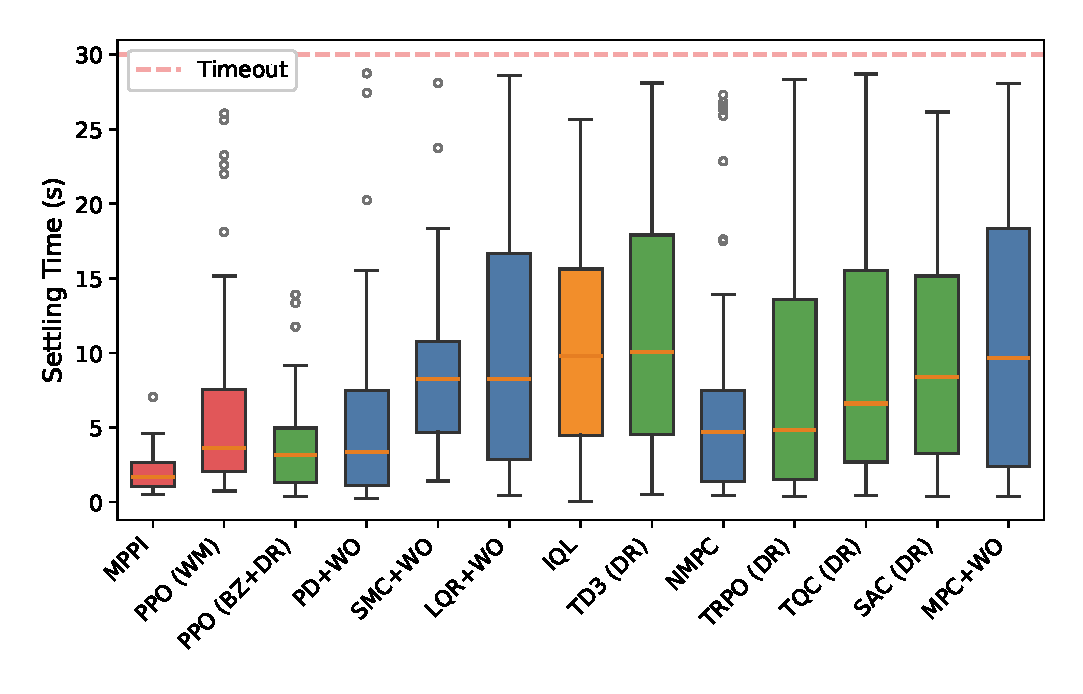
\includegraphics[width=0.95\columnwidth]{figures/exp1_boxplot.eps}
  \caption{Settling time distributions. MPPI shows the tightest
    distribution with no outliers beyond 9\,s. Classical controllers
    with wall override show bimodal behavior: fast successes plus
    occasional slow recoveries after the override triggers.}
  \label{fig:boxplot}
\end{figure}

\begin{figure}[t]
  \centering
  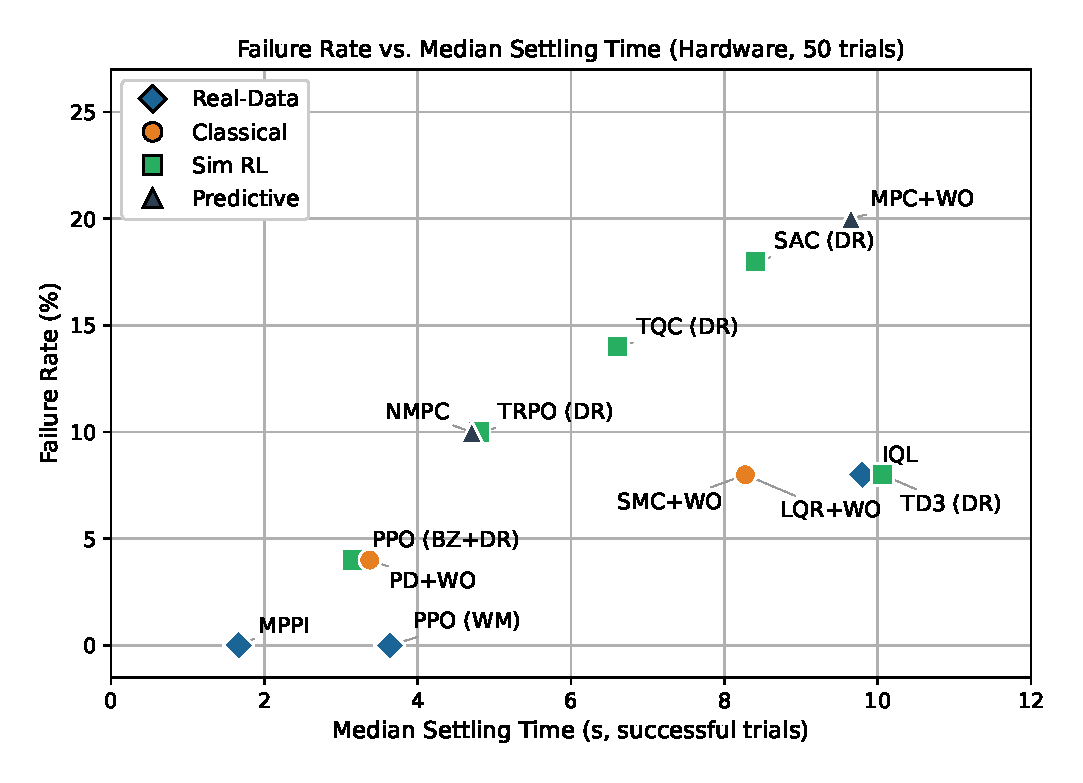
\includegraphics[width=0.95\columnwidth]{figures/hw_sr_vs_settling.eps}
  \caption{Failure rate versus median settling time (successful
    trials) across all 13 controllers. Both axes increase toward worse
    outcomes, so the ideal corner is bottom-left. MPPI ties for the best
    success rate and is fastest on median settling (100\%, 1.67\,s). Two
    controllers achieve perfect reliability; all handle the boundary,
    whether explicitly or through learned dynamics.}
  \label{fig:pareto}
\end{figure}

\subsection{The Reach of Domain Randomization}

Domain randomization is the workhorse of sim-to-real transfer~\cite{zhao2020simtoreal}, and has carried policies onto hardware as demanding as in-hand manipulation and champion-level drone racing.
In our PPO ablation it does most of the work and then plateaus: it lifts hardware success from 60\% without it to 90\% with it, a thirty-point gain, after which the remaining gap did not close with more of it.

The source of the remaining gap is less certain.
We can model one sensor effect directly: near the arc edges the ToF sensors saturate and report frozen values, and a policy trained without this artifact overcorrects on stale data.
Adding a blind-zone model lifts PPO from 90\% to 98\%.\footnote{The domain-randomization and blind-zone ablations in this subsection are measured within the S-curve servo-model family, the regime the extended training runs used. Tbl.~\ref{tab:results} instead reports PPO~(BZ+DR) at the first-order-lag checkpoint (96\%), matched to the servo model the other 4 RL agents trained against so the cross-agent comparison is fair; the supplement reports both.} At 50 trials this eight-point move is within the benchmark's resolution, so we treat the perceptual reading as a hypothesis; the data cannot yet resolve an effect this small.
Nor is modeling the sensor the only route past the plateau: trained to 5M steps, the base PPO policy also reaches 100\% over 50 hardware trials, so the blind-zone model is the training-efficient path rather than the necessary one.
It fits what we see: the five simulation-trained RL agents all reach 96--100\% in simulation yet span only 82\% to 96\% on hardware, though they also differ in their training conditions, so this cross-agent spread is suggestive and not conclusive.

\subsection{A Note on Offline RL}

IQL achieves 92\% success at the second-lowest control effort of any controller (0.395 RMS, behind only MPPI), using no simulator: its conservative policy is reliable and gentle on the hardware, at the price of speed, with a median settling of 9.80\,s, roughly six times MPPI's.
The result is attractive mainly for where the data came from: the dataset built up as a by-product of normal evaluation runs, so once a platform is instrumented and several controllers have been run, offline RL becomes a viable low-overhead option when simulation fidelity is uncertain.

\section{Discussion and Conclusions}
\label{sec:discussion}

The controller choice posed at the outset has a conditional answer on this system.
A practitioner who can gather hardware logs and afford real-time CPU rollouts should consider planning through a learned model: MPPI ties for the top success rate and settles fastest (100\%, 1.67\,s median).
Reliability alone, however, cannot decide among the leaders: at 50 trials per controller the top group is statistically inseparable on success rate, and even MPPI's settling advantage, significant over nine of the twelve other controllers, does not separate it from PD+WO, PPO~(BZ+DR), or NMPC.
The choice among the reliable controllers rests on the axes that do differ: settling consistency, control effort, deploy-time compute, and the engineering a team already has in place.
Effort is one such axis the benchmark can resolve statistically, and there MPPI and IQL are significantly better than the remaining eleven.

The engineering axis is the one most directly relevant to the classical result.
An already running linear regulator can reach reliable hardware success on this system simply by handling the boundary constraint: the wall override alone lifted nominal LQR from 20\% to 92\% success.
It follows that, for reliability in a constrained system like ours, the choice between a classical and a learned controller matters less than the decision to model the boundary at all.

% For a practitioner the
% classical-versus-learned decision, which absorbs a great deal of
% attention, matters less for reliability on a constrained system like ours than
% whether the boundary is handled at all, by a rule any of these controllers
% can carry. We did not expect the four paradigms to sit this close together
% on hardware, and their convergence once the boundary was handled surprised
% us more than any single ranking.

MPPI has a higher settling speed due to three mechanisms acting together: a model learned from hardware logs bridges the sim-to-real gap, sampling-based planning handles the boundary problem without a manual override, and replanning at every step absorbs the model error that remains.
The drawbacks are the real-time CPU rollouts at every control period and a non-trivial tuning effort.

We observe that the various approaches merely shift the engineering effort rather than remove it: analytical controllers need modeling and tuning, simulation-trained RL needs a simulator with credible sensor and motor models, offline RL needs logged trials, and model-based planning needs exploration data and a trained dynamics model.
Therefore choosing among the reliable controllers is essentially choosing which of these inputs is most readily available.

% MPPI earns its speed from three properties working together: a model
% learned from hardware logs sidesteps the sim-to-real gap, sampling-based
% planning keeps rollouts clear of the rail without a hand-written override,
% and replanning at every step absorbs the model error that remains. The
% price is real-time CPU rollouts at every control period, plus a tuning
% effort that was not trivial. The approaches
% shift the engineering effort rather than remove it: analytical controllers
% need modeling and tuning, simulation-trained RL needs a simulator with
% credible sensor and motor models, offline RL needs logged trials, and
% model-based planning needs exploration data and a trained dynamics model.
% A team choosing among the reliable controllers is really choosing which of
% these inputs it can most readily produce.

Our results suggest a pragmatic order of priorities for deploying a controller on a constrained system.
One should begin with explicit constraint handling, the largest single lever on reliability we measured, worth 72 to 80 percentage points across the three classical controllers, whether through a boundary heuristic like our wall override or a formal method such as a control barrier function~\cite{ames2019control}.
Where simulation fidelity is uncertain, logged hardware data deserves to be treated as a serious alternative to building a simulator: the three controllers built from it take the two highest success rates and the two lowest control efforts in the benchmark, and IQL's dataset accumulated as a by-product of ordinary evaluation runs rather than a dedicated collection.
And once a policy is deployed, on-robot fine-tuning should not be counted on to rescue it.
Over 50,000 hardware steps per policy, and with a noise-free reward signal that simulation cannot supply, fine-tuning left the world-model policy unchanged at 100\% and nominally degraded both simulation-trained agents, though those two arms rest on ten trials each; the supplement's fine-tuning appendix reports the study.

One further observation reinforces the caution about simulation, which is that simulation rank does not forecast hardware rank: SAC balanced perfectly and settled quickly in simulation yet was the least reliable of the five on hardware, at 82\%, with only MPC+WO, at 80\%, ranking lower overall.
With a single algorithm trained under its own conditions we only take this as a caution to bear in mind; our data do not establish it as a controlled effect.

\subsection{Limitations and Future Work}

These results are specific to our system: the quantitative ranking applies to this particular arc geometry, sensor characteristics, and control frequency, and it may shift on systems without hard constraint boundaries or with faster dynamics.
Two rankings also depend on configuration choices documented in the supplement: PPO-WM's world model is trained on one of two logged collections whose data properties suit RL training, and the simulation-trained agents did not all use the same sensor model, since PPO~(BZ+DR) includes a blind-zone model the other four omit.
The reinforcement-learning results are also single-seed: each agent was trained once (seed~1), so we report point estimates and do not characterize the training-stochasticity variance that a multi-seed study would expose.
The families also differ in more than paradigm, in data source, model fidelity, tuning effort, boundary mechanism, and deploy-time compute, so we read the small cross-paradigm spread as constraint handling being decisive in this configuration rather than as an isolation of paradigm as a causal variable.

We offer the qualitative findings, constraint awareness as the dominant lever, the training efficiency of modeling the dominant sensor failure, and the viability of real-data model-based planning, as conjectures to test on similar constrained underactuated systems; we make no claim for them beyond this platform.

Natural next directions are to expand the platform toward more axes and higher dimensionality with a modified constraint structure, moving toward more complex underactuated systems, and to investigate uncertainty-aware exploration as an alternative to random data collection.


\section*{Acknowledgment}
The authors thank the Fraunhofer IIS team for hardware support.

\bibliographystyle{IEEEtran}
\bibliography{bibliography}

\end{document}
